\documentclass[aspectratio=169]{beamer}

\usetheme[progressbar=foot,block=fill,sectionpage=none,numbering=fraction]{metropolis}
\usefonttheme{professionalfonts}
\usepackage[sfdefault,condensed]{roboto}
\usepackage{roboto-mono}
\usepackage{amsmath,amssymb,mathtools}
\usepackage{unicode-math}
\setmathfont{Libertinus Math}
\usepackage{tikz}
\usetikzlibrary{arrows.meta,calc,fit,positioning,shapes.geometric}
\usepackage{booktabs}
\usepackage{array}
\usepackage{hyperref}
\usepackage{microtype}

\definecolor{ink}{HTML}{242832}
\definecolor{paper}{HTML}{FBFAF7}
\definecolor{muted}{HTML}{747B88}
\definecolor{line}{HTML}{DDE2EA}
\definecolor{accent}{HTML}{356AE6}
\definecolor{accentdark}{HTML}{204DB6}
\definecolor{accentlite}{HTML}{EAF0FF}
\definecolor{green}{HTML}{257A63}
\definecolor{greenlite}{HTML}{E2F1EA}
\definecolor{blue}{HTML}{356AE6}
\definecolor{bluelite}{HTML}{EAF0FF}
\definecolor{amber}{HTML}{B7791F}
\definecolor{amberlite}{HTML}{FFF1D6}
\definecolor{red}{HTML}{B84A45}
\definecolor{redlite}{HTML}{F8E4E1}
\definecolor{violet}{HTML}{7356A3}

\setbeamercolor{normal text}{fg=ink,bg=paper}
\setbeamercolor{alerted text}{fg=red}
\setbeamercolor{example text}{fg=green}
\setbeamercolor{frametitle}{fg=ink,bg=paper}
\setbeamercolor{title}{fg=ink}
\setbeamercolor{subtitle}{fg=muted}
\setbeamercolor{progress bar}{fg=accent,bg=line}
\setbeamercolor{block title}{fg=ink,bg=accentlite}
\setbeamercolor{block body}{fg=ink,bg=white}
\setbeamercolor{footnote}{fg=muted}
\setbeamertemplate{navigation symbols}{}
\setbeamertemplate{frame numbering}[fraction]
\setbeamerfont{title}{size=\fontsize{24}{28},series=\bfseries}
\setbeamerfont{subtitle}{size=\large,series=\bfseries}
\setbeamerfont{frametitle}{size=\Large,series=\bfseries}
\setbeamerfont{normal text}{size=\small}
\setbeamerfont{footnote}{size=\tiny}

\newcommand{\source}[1]{\par\vspace{0.08em}{\tiny\color{muted}#1}}
\newcommand{\tagbox}[2]{\colorbox{#1}{\scriptsize\strut\hspace{0.35em}#2\hspace{0.35em}}}
\newcommand{\kicker}[1]{{\scriptsize\color{accent}\bfseries\MakeUppercase{#1}}}

\title[From Papers to Math Contracts]{From Papers to Math\\Contracts}
\subtitle{AgtXIv / MathContractRegistry: auditable claim reuse}
\author{Math-first pilot}
\date{2026}

\setbeamertemplate{title page}{%
  \begin{tikzpicture}[remember picture,overlay]
    \fill[paper] (current page.south west) rectangle (current page.north east);
    \fill[accent]
      ([xshift=-0.40\paperwidth]current page.south east) --
      (current page.south east) -- (current page.north east) --
      ([xshift=-0.31\paperwidth]current page.north east) -- cycle;
    \fill[accentdark,opacity=0.30]
      ([xshift=-0.29\paperwidth]current page.south east) --
      (current page.south east) -- (current page.north east) --
      ([xshift=-0.17\paperwidth]current page.north east) -- cycle;

    \node[anchor=north west] at ([xshift=0.07\paperwidth,yshift=-0.11\paperheight]current page.north west) {%
      \begin{minipage}{0.58\paperwidth}
        \kicker{Verification-aware scientific publishing}\par
        \vspace{1.0em}
        {\usebeamerfont{title}\usebeamercolor[fg]{title}\inserttitle\par}
        \vspace{0.45em}
        {\usebeamerfont{subtitle}\usebeamercolor[fg]{subtitle}\insertsubtitle\par}
        \vspace{1.1em}
        {\color{accent}\rule{2.2cm}{1.1pt}}\par
        \vspace{1.2em}
        {\bfseries\insertauthor}\par
        \vspace{0.15em}
        {\color{muted}AgtXIv / MathContractRegistry\quad/\quad\insertdate}
      \end{minipage}
    };

    \node[anchor=center] at ([xshift=-0.17\paperwidth]current page.east) {%
      \begin{tikzpicture}[node distance=0.48cm]
        \node[rounded corners=2pt,draw=white,fill=white,fill opacity=0.12,text opacity=1,
          text=white,minimum width=3.0cm,minimum height=0.72cm,align=center] (pdf)
          {paper + code};
        \node[rounded corners=2pt,draw=white,fill=white,fill opacity=0.12,text opacity=1,
          text=white,minimum width=3.0cm,minimum height=0.72cm,align=center,below=of pdf] (agent)
          {paper agent};
        \node[rounded corners=2pt,draw=white,fill=white,fill opacity=0.18,text opacity=1,
          text=white,minimum width=3.0cm,minimum height=0.72cm,align=center,below=of agent] (contract)
          {MathContract};
        \draw[->,white,thick] (pdf) -- (agent);
        \draw[->,white,thick] (agent) -- (contract);
      \end{tikzpicture}
    };
  \end{tikzpicture}%
}

\begin{document}

\maketitle

\section{Motivation}

\begin{frame}{Start with a concrete promise}
  \begin{center}
    {\Large For a theorem query, return more than a list of ``related papers'':}\\[0.55em]
    {\color{green}\LARGE\textbf{an auditable, reusable dependency path with gaps marked.}}
  \end{center}
  \vspace{1.1em}
  \begin{columns}[T,onlytextwidth]
    \column{0.31\textwidth}
      \centering\tagbox{greenlite}{target address}\\[0.35em]
      \scriptsize where the target claim lives in the registry
    \column{0.31\textwidth}
      \centering\tagbox{bluelite}{dependency path}\\[0.35em]
      \scriptsize which definitions, assumptions, and theorems it actually uses
    \column{0.31\textwidth}
      \centering\tagbox{amberlite}{frontier + delta}\\[0.35em]
      \scriptsize connected evidence, unresolved boundary, and new work needed
  \end{columns}
  \source{Core object: a reasoning-centric, versioned, claim-level MathContract.}
\end{frame}

\begin{frame}{Reading bandwidth becomes the bottleneck}
  \begin{columns}[T,onlytextwidth]
    \column{0.52\textwidth}
      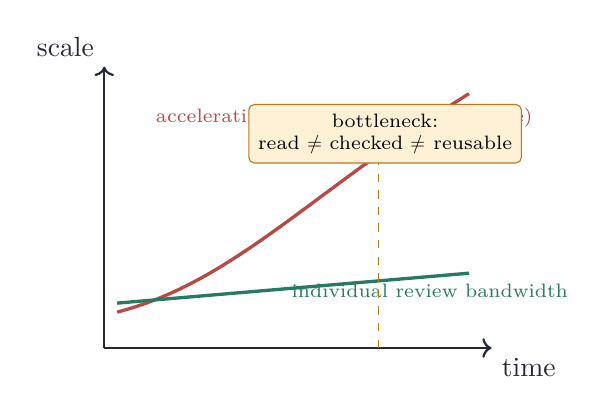
\begin{tikzpicture}[x=0.82cm,y=0.76cm]
        \draw[->,thick,ink] (0,0) -- (6.0,0) node[below right]{time};
        \draw[->,thick,ink] (0,0) -- (0,4.7) node[above left]{scale};
        \draw[very thick,red] (0.2,0.6) .. controls (2.0,1.1) and (3.2,2.6) .. (5.65,4.25);
        \draw[very thick,green] (0.2,0.75) -- (5.65,1.25);
        \node[anchor=west,font=\scriptsize\color{red},align=left] at (0.65,3.85)
          {accelerating accumulation\;(illustrative)};
        \node[anchor=west,font=\scriptsize\color{green},align=left] at (2.75,0.95)
          {individual review bandwidth};
        \draw[dashed,amber] (4.25,0) -- (4.25,3.25);
        \node[fill=amberlite,draw=amber,rounded corners=2pt,align=center,font=\scriptsize] at (4.35,3.58)
          {bottleneck:\\read $\neq$ checked $\neq$ reusable};
      \end{tikzpicture}
    \column{0.44\textwidth}
      \vspace{0.5em}
      \begin{itemize}\setlength{\itemsep}{0.55em}
        \item Finding a paper is no longer the hard part.
        \item Harder: which results can later work safely rely on?
        \item A reader must track \textbf{definitions, quantifiers, domains, proof dependencies, and counterexamples}.
      \end{itemize}
      \vspace{0.4em}
      \colorbox{greenlite}{\parbox{0.95\linewidth}{\centering\textbf{AgtXIv changes the unit of reading:}\\from a whole PDF to an inspectable mathematical interface.}}
  \end{columns}
  \source{Qualitative sketch only; no unsupported numerical growth claim is used.}
\end{frame}

\begin{frame}{A citation graph is not a proof graph}
  \begin{columns}[T,onlytextwidth]
    \column{0.32\textwidth}
      \centering\textbf{Citation graph}\par\vspace{0.3em}
      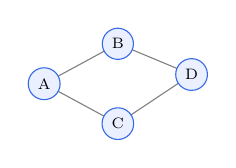
\begin{tikzpicture}[>=Latex,scale=0.78,transform shape]
        \draw[->,gray] (0,0) -- (1.2,0.65);
        \draw[->,gray] (0,0) -- (1.2,-0.65);
        \draw[->,gray] (1.2,0.65) -- (2.4,0.15);
        \draw[->,gray] (1.2,-0.65) -- (2.4,0.15);
        \foreach \p/\t in {(0,0)/A,(1.2,0.65)/B,(1.2,-0.65)/C,(2.4,0.15)/D}
          \node[circle,fill=bluelite,draw=blue,inner sep=2.5pt] at \p {\scriptsize\t};
      \end{tikzpicture}
      \scriptsize Paper $A$ cites $B$, but for what reason?
    \column{0.32\textwidth}
      \centering\textbf{Scientific claim graph}\par\vspace{0.3em}
      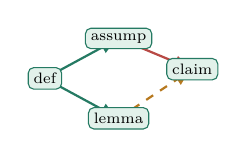
\begin{tikzpicture}[>=Latex,scale=0.78,transform shape]
        \draw[->,thick,green] (0,0) -- (1.2,0.65);
        \draw[->,thick,green] (0,0) -- (1.2,-0.65);
        \draw[->,thick,red] (1.2,0.65) -- (2.4,0.15);
        \draw[->,thick,amber,dashed] (1.2,-0.65) -- (2.4,0.15);
        \foreach \p/\t in {(0,0)/def,(1.2,0.65)/assump,(1.2,-0.65)/lemma,(2.4,0.15)/claim}
          \node[rounded corners=2pt,fill=greenlite,draw=green,inner sep=2.5pt] at \p {\scriptsize\t};
      \end{tikzpicture}
      \scriptsize Which premises does the claim actually use?
    \column{0.32\textwidth}
      \centering\textbf{Lean support graph}\par\vspace{0.3em}
      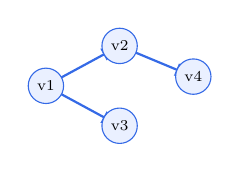
\begin{tikzpicture}[>=Latex,scale=0.78,transform shape]
        \draw[->,thick,blue] (0,0) -- (1.2,0.65);
        \draw[->,thick,blue] (0,0) -- (1.2,-0.65);
        \draw[->,thick,blue] (1.2,0.65) -- (2.4,0.15);
        \foreach \p/\t in {(0,0)/v1,(1.2,0.65)/v2,(1.2,-0.65)/v3,(2.4,0.15)/v4}
          \node[circle,fill=bluelite,draw=blue,inner sep=2.5pt] at \p {\scriptsize\t};
      \end{tikzpicture}
      \scriptsize Which declarations were checked in a fixed environment?
  \end{columns}
  \vspace{0.9em}
  \begin{center}
    \colorbox{redlite}{\parbox{0.82\linewidth}{\centering\textbf{A cites B} $\;\not\Rightarrow\;$ A uses a theorem from B, or that B's assumptions hold.}}
  \end{center}
  \source{AgtXIv tracks provenance, mathematical dependencies, Lean support, and separate computational and physical evidence.}
\end{frame}

\begin{frame}{Automated semantic extraction creates false edges}
  \begin{center}
    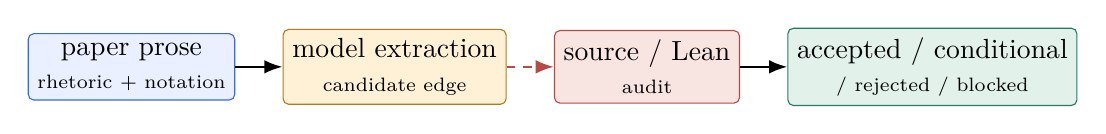
\begin{tikzpicture}[>=Latex,node distance=0.55cm and 0.6cm]
      \node[rounded corners=2pt,draw=blue,fill=bluelite,minimum width=2.25cm,minimum height=0.8cm,align=center] (prose) {paper prose\\\scriptsize rhetoric + notation};
      \node[rounded corners=2pt,draw=amber,fill=amberlite,minimum width=2.35cm,minimum height=0.8cm,align=center,right=of prose] (llm) {model extraction\\\scriptsize candidate edge};
      \node[rounded corners=2pt,draw=red,fill=redlite,minimum width=2.35cm,minimum height=0.8cm,align=center,right=of llm] (audit) {source / Lean\\\scriptsize audit};
      \node[rounded corners=2pt,draw=green,fill=greenlite,minimum width=2.35cm,minimum height=0.8cm,align=center,right=of audit] (state) {accepted / conditional\\\scriptsize / rejected / blocked};
      \draw[->,thick] (prose) -- (llm);
      \draw[->,thick,dashed,red] (llm) -- (audit);
      \draw[->,thick] (audit) -- (state);
    \end{tikzpicture}
  \end{center}
  \vspace{0.55em}
  \begin{columns}[T,onlytextwidth]
    \column{0.48\textwidth}
      \begin{itemize}\setlength{\itemsep}{0.25em}
        \item rhetorical overstatement or missing assumptions
        \item notation, quantifier, or domain mismatch
        \item background citation misread as a load-bearing dependency
      \end{itemize}
    \column{0.48\textwidth}
      \begin{itemize}\setlength{\itemsep}{0.25em}
        \item honest intermediate mistakes or literature disputes
        \item hidden counterexamples or errata
        \item a model can inherit only the text it reads
      \end{itemize}
  \end{columns}
  \vspace{0.2em}
  \centering\small\textbf{Therefore the first graph is}\;\tagbox{amberlite}{ORACLE\_PROPOSED / CANDIDATE}\;\textbf{and cannot promote itself to accepted.}
  \source{Current edge evidence remains Oracle-proposed, unreviewed at edge level, and candidate.}
\end{frame}

\begin{frame}{Formal physics infrastructure is becoming usable}
  \begin{columns}[T,onlytextwidth]
    \column{0.58\textwidth}
      \footnotesize
      \renewcommand{\arraystretch}{1.06}
      \begin{tabular}{@{}p{0.66\linewidth}p{0.25\linewidth}@{}}
        \toprule
        \textbf{Representative direction} & \textbf{arXiv}\tabularnewline
        \midrule
        HepLean & 2405.08863\\
        Physics index notation & 2411.07667\\
        PhysProver & 2601.15737\\
        MerLean & 2602.16554\\
        Lean-QEC & 2605.16523\\
        TNLean & 2607.07857\\
        Lean-QIT & 2607.09632\\
        Axioms / Seiberg--Witten & 2607.06379\\
        \bottomrule
      \end{tabular}
    \column{0.38\textwidth}
      \vspace{0.2em}
      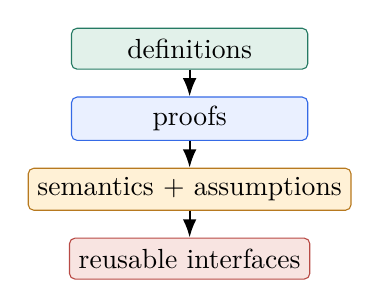
\begin{tikzpicture}[>=Latex,node distance=0.34cm]
        \node[rounded corners=2pt,fill=greenlite,draw=green,minimum width=3.0cm,minimum height=0.52cm,align=center] (d) {definitions};
        \node[rounded corners=2pt,fill=bluelite,draw=blue,minimum width=3.0cm,minimum height=0.52cm,align=center,below=of d] (p) {proofs};
        \node[rounded corners=2pt,fill=amberlite,draw=amber,minimum width=3.0cm,minimum height=0.52cm,align=center,below=of p] (s) {semantics + assumptions};
        \node[rounded corners=2pt,fill=redlite,draw=red,minimum width=3.0cm,minimum height=0.52cm,align=center,below=of s] (r) {reusable interfaces};
        \draw[->,thick] (d) -- (p);
        \draw[->,thick] (p) -- (s);
        \draw[->,thick] (s) -- (r);
      \end{tikzpicture}
      \vspace{0.25em}
      \scriptsize Intuition: formalization is not merely formula-to-code translation; it exposes missing premises, intent drift, and broken literature bridges.
  \end{columns}
  \source{arXiv identifiers checked; kernel-checked proofs still need alignment with the intended statement.}
\end{frame}

\section{From PDF to contracts}

\begin{frame}{A paper agent turns a static PDF into a callable object}
  \begin{columns}[T,onlytextwidth]
    \column{0.29\textwidth}
      \centering\tagbox{redlite}{PDF}\par\vspace{0.5em}
      
\begin{tikzpicture}
        \draw[fill=white,draw=red,thick,rounded corners=2pt] (0,0) rectangle (2.25,2.55);
        \draw[red,thick] (0.3,2.05) -- (1.95,2.05);
        \foreach \y in {1.65,1.35,1.05,0.75,0.45}
          \draw[line] (0.3,\y) -- (1.95,\y);
      \end{tikzpicture}
      \scriptsize narrative, figures, and citations\\are hard to call or reuse directly
    \column{0.34\textwidth}
      \centering\tagbox{amberlite}{APP}\par\vspace{0.5em}
      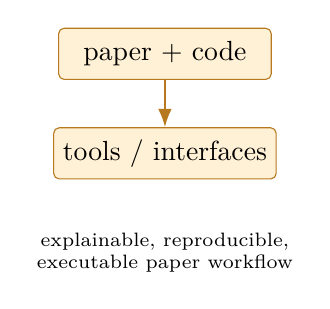
\begin{tikzpicture}[>=Latex]
        \node[rounded corners=2pt,fill=amberlite,draw=amber,minimum width=2.7cm,minimum height=0.65cm] (src) {paper + code};
        \node[rounded corners=2pt,fill=amberlite,draw=amber,minimum width=2.7cm,minimum height=0.65cm,below=0.6cm of src] (mcp) {tools / interfaces};
        \draw[->,thick,amber] (src) -- (mcp);
        \node[font=\scriptsize,align=center,below=0.55cm of mcp] {explainable, reproducible,\\executable paper workflow};
      \end{tikzpicture}
    \column{0.31\textwidth}
      \centering\tagbox{greenlite}{AgtXIv}\par\vspace{0.5em}
      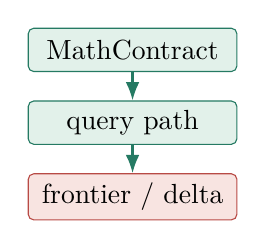
\begin{tikzpicture}[>=Latex,node distance=0.36cm]
        \node[rounded corners=2pt,fill=greenlite,draw=green,minimum width=2.65cm,minimum height=0.55cm] (c) {MathContract};
        \node[rounded corners=2pt,fill=greenlite,draw=green,minimum width=2.65cm,minimum height=0.55cm,below=of c] (q) {query path};
        \node[rounded corners=2pt,fill=redlite,draw=red,minimum width=2.65cm,minimum height=0.55cm,below=of q] (f) {frontier / delta};
        \draw[->,thick,green] (c) -- (q);
        \draw[->,thick,green] (q) -- (f);
      \end{tikzpicture}
  \end{columns}
  \vspace{0.2em}
  \begin{center}
    Sirui Lu and Xiao-Liang Qi's \textbf{Agentic Publication Protocol (APP)}\;\href{https://arxiv.org/abs/2606.27386}{\texttt{arXiv:2606.27386}}\\
    \scriptsize\color{muted}packages a versioned repository, code, data, environment, and \texttt{AGENTS.md} as one publication object. AgtXIv adds claim-level evidence for why a result can be inherited.
  \end{center}
  \begin{center}
    \tiny\color{muted}Related direction: Paper2Agent, \href{https://arxiv.org/abs/2509.06917}{\texttt{arXiv:2509.06917}}.
  \end{center}
\end{frame}

\begin{frame}{APP makes a repository a stable publication object}
  \begin{center}
    \kicker{Definition}\qquad
    \textbf{publication object = public git repository + a specific release}
  \end{center}
  \vspace{0.18em}
  \begin{columns}[T,onlytextwidth]
    \column{0.40\textwidth}
      \textbf{Three layers}
      \vspace{0.12em}
      \colorbox{bluelite}{\parbox[c][0.66cm][c]{4.08cm}{\scriptsize\textbf{1. Human publication}\\[-0.1em]\tiny manuscript / README / license / code / data / environment}}\\[-0.02em]
      \centering\textcolor{muted}{$\downarrow$}\\[-0.08em]
      \colorbox{amberlite}{\parbox[c][0.66cm][c]{4.08cm}{\scriptsize\textbf{2. Agent-facing layer}\\[-0.1em]\tiny \texttt{AGENTS.md}: ground truth / navigation / setup}}\\[-0.02em]
      \centering\textcolor{muted}{$\downarrow$}\\[-0.08em]
      \colorbox{greenlite}{\parbox[c][0.66cm][c]{4.08cm}{\scriptsize\textbf{3. Release + verification}\\[-0.1em]\tiny tag / commit-tree hash / manifest / author approval}}\\[-0.02em]
      \centering\tiny\color{muted}contents / operator manual / version seal
    \column{0.57\textwidth}
      \textbf{Five-step \texttt{publish-paper} flow}\par\vspace{-0.1em}
      \kicker{run / pack / instruct / inspect / seal}
      \vspace{0.05em}
      {\scriptsize
      \renewcommand{\arraystretch}{0.86}
      \begin{tabular}{@{}>{\color{accent}\bfseries}r@{\quad}p{3.05cm}@{\quad}p{2.35cm}@{}}
        1 & \texttt{reproduce-results} & \tiny reproduction report \\
        2 & \texttt{prepare-staging} & \tiny organized public tree \\
        3 & \texttt{define-paper-agent} & \tiny concise \texttt{AGENTS.md} \\
        4 & \texttt{validate-publication} & \tiny structural + usability checks \\
        5 & \texttt{release-outcome} & \tiny approved tag + manifest \\
      \end{tabular}}
      \vspace{0.08em}
      \parbox{5.8cm}{\centering\tiny\color{muted}The detailed records distinguish reproduced, blocked, manual-only, inconsistent, and privacy or path failures.}
  \end{columns}
  \vspace{0.12em}
  \centering\colorbox{accentlite}{\parbox{0.92\linewidth}{\centering\tiny Validation checks structure, metadata, and reader usability; it is not peer review or a certificate of scientific truth. \textbf{AgtXIv adds claim-level dependencies and evidence on top.}}}
  \vspace{0.04em}
  \begin{center}
    \tiny\color{muted}Sirui Lu and Xiao-Liang Qi, Agentic Publication Protocol, \href{https://arxiv.org/abs/2606.27386}{\texttt{arXiv:2606.27386}}.
  \end{center}
\end{frame}

\begin{frame}{A query should return a path receipt}
  \begin{center}
    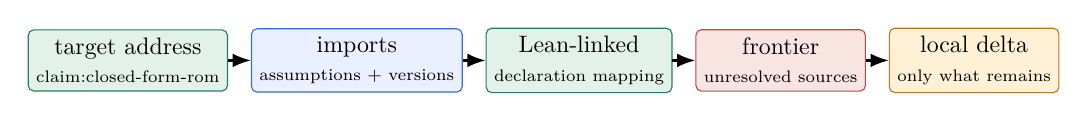
\begin{tikzpicture}[>=Latex,node distance=0.65cm and 0.34cm,scale=0.86,transform shape]
      \node[rounded corners=2pt,fill=greenlite,draw=green,minimum width=2.4cm,minimum height=0.75cm,align=center] (a) {target address\\\scriptsize claim:closed-form-rom};
      \node[rounded corners=2pt,fill=bluelite,draw=blue,minimum width=2.4cm,minimum height=0.75cm,align=center,right=of a] (b) {imports\\\scriptsize assumptions + versions};
      \node[rounded corners=2pt,fill=greenlite,draw=green,minimum width=2.4cm,minimum height=0.75cm,align=center,right=of b] (c) {Lean-linked\\\scriptsize declaration mapping};
      \node[rounded corners=2pt,fill=redlite,draw=red,minimum width=2.4cm,minimum height=0.75cm,align=center,right=of c] (d) {frontier\\\scriptsize unresolved sources};
      \node[rounded corners=2pt,fill=amberlite,draw=amber,minimum width=2.4cm,minimum height=0.75cm,align=center,right=of d] (e) {local delta\\\scriptsize only what remains};
      \foreach \u/\v in {a/b,b/c,c/d,d/e}{\draw[->,thick] (\u) -- (\v);}
    \end{tikzpicture}
  \end{center}
  \vspace{1.0em}
  \begin{columns}[T,onlytextwidth]
    \column{0.49\textwidth}
      \textbf{Auditable fields in the current registry}
      \begin{itemize}\setlength{\itemsep}{0.32em}
        \item normalized statement, quantifiers, domain, and exactness
        \item source anchors, imports, and verification references
        \item Lean declaration, blockers, and versions
      \end{itemize}
    \column{0.49\textwidth}
      \textbf{Not acceptable}
      \begin{itemize}\setlength{\itemsep}{0.32em}
        \item returning only a list of ``related papers''
        \item describing a candidate edge as an accepted dependency
        \item using fluent prose to hide a missing premise
      \end{itemize}
  \end{columns}
  \source{A MathContract is a reusable mathematical interface with assumptions, sources, formal links, and evidence state.}
\end{frame}

\begin{frame}{Physical picture: a measurement window sees only a shadow}
  \begin{columns}[T,onlytextwidth]
    \column{0.46\textwidth}
      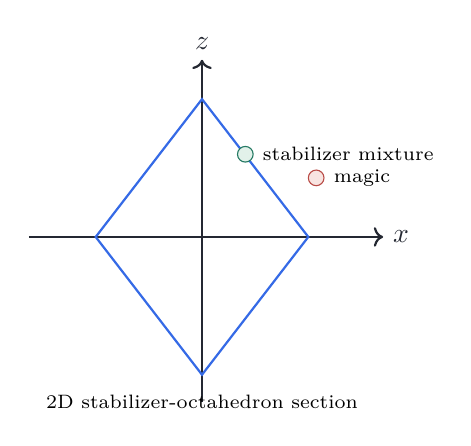
\begin{tikzpicture}[x=1.0cm,y=1.0cm]
        \draw[->,thick,ink] (-2.2,0) -- (2.3,0) node[right]{$x$};
        \draw[->,thick,ink] (0,-2.1) -- (0,2.25) node[above]{$z$};
        \draw[thick,blue] (0,1.75) -- (1.35,0) -- (0,-1.75) -- (-1.35,0) -- cycle;
        \node[fill=greenlite,draw=green,circle,inner sep=2pt] (p) at (0.55,1.05) {};
        \node[font=\scriptsize,anchor=west] at (0.65,1.05) {stabilizer mixture};
        \node[fill=redlite,draw=red,circle,inner sep=2pt] (m) at (1.45,0.75) {};
        \node[font=\scriptsize,anchor=west] at (1.55,0.75) {magic};
        \node[font=\scriptsize,anchor=north] at (0,-1.88) {2D stabilizer-octahedron section};
      \end{tikzpicture}
    \column{0.50\textwidth}
      \begin{itemize}\setlength{\itemsep}{0.22em}
        \item Six Pauli eigenstates form the one-qubit stabilizer octahedron.
        \item A small measurement window casts a shadow of the full polytope.
        \item Outside: a sound magic certificate.\\Inside: unobserved magic may remain.
        \item RoM is the minimum $l_1$ cost of a signed decomposition, not a Euclidean distance.
      \end{itemize}
  \end{columns}
  \vspace{0.02em}
  \colorbox{accentlite}{\parbox{0.92\linewidth}{\centering\scriptsize\textbf{$G_M$ is a different object:}\;vertices are Pauli operators, edges mean anticommutation, and independent sets are commuting contexts.}}
\end{frame}

\section{A concrete registry slice}

\begin{frame}{Concrete query: from a measurement window to a closed form}
  \begin{center}
    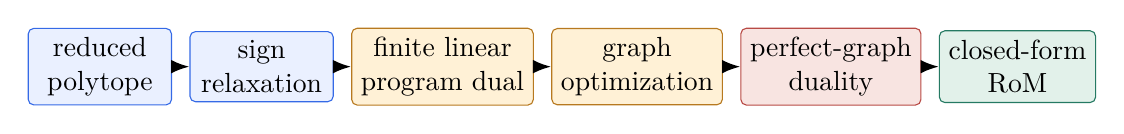
\begin{tikzpicture}[>=Latex,node distance=0.55cm and 0.22cm]
      \node[rounded corners=2pt,fill=bluelite,draw=blue,minimum width=1.82cm,minimum height=0.62cm,align=center] (v) {reduced\\polytope};
      \node[rounded corners=2pt,fill=bluelite,draw=blue,minimum width=1.82cm,minimum height=0.62cm,align=center,right=of v] (s) {sign\\relaxation};
      \node[rounded corners=2pt,fill=amberlite,draw=amber,minimum width=1.82cm,minimum height=0.62cm,align=center,right=of s] (l) {finite linear\\program dual};
      \node[rounded corners=2pt,fill=amberlite,draw=amber,minimum width=1.82cm,minimum height=0.62cm,align=center,right=of l] (g) {graph\\optimization};
      \node[rounded corners=2pt,fill=redlite,draw=red,minimum width=1.82cm,minimum height=0.62cm,align=center,right=of g] (p) {perfect-graph\\duality};
      \node[rounded corners=2pt,fill=greenlite,draw=green,minimum width=1.82cm,minimum height=0.62cm,align=center,right=of p] (t) {closed-form\\RoM};
      \foreach \u/\vv in {v/s,s/l,l/g,g/p,p/t}{\draw[->,thick] (\u) -- (\vv);}
    \end{tikzpicture}
  \end{center}
  \vspace{0.85em}
  \begin{block}{Question in plain language}
    Why, when there is no Pauli-active dependency and $G_M$ is a perfect graph, does
    $\mathrm{RoM}_M(\rho)=\max\!\left(1,\max_Q\sum_{P\in Q}|\operatorname{tr}(P\rho)|\right)$?
  \end{block}
  \vspace{0.35em}
  \begin{columns}[T,onlytextwidth]
    \column{0.48\textwidth}
      \small\tagbox{greenlite}{inherited}\;stabilizer form, projection semantics, selected local Lean declarations
    \column{0.48\textwidth}
      \small\tagbox{redlite}{unresolved frontier}\;weighted perfect-graph duality, finite linear-program strong duality, source alignment
  \end{columns}
  \source{Target contract: \texttt{claim:closed-form-rom}; current state: LOCAL\_DERIVATION\_WITH\_BLOCKED\_IMPORTS.}
\end{frame}

\begin{frame}{The registry is explicit about what remains unverified}
  \begin{columns}[T,onlytextwidth]
    \column{0.48\textwidth}
      \begin{tabular}{@{}lr@{}}
        \toprule
        whole-paper nodes & 74\\
        mathematical interfaces & 65\\
        mapped Paper Agents & 5\\
        typed candidate edges (demo) & 114\\
        unresolved external interfaces & 8\\
        \bottomrule
      \end{tabular}
      \vspace{0.55em}
      \parbox[t]{0.95\linewidth}{\scriptsize The canonical whole-paper graph has 129 edges; the demo keeps 114 edges between mathematical interfaces.}
    \column{0.48\textwidth}
      \begin{tabular}{@{}lr@{}}
        \toprule
        Lean-linked declarations & 10\\
        GAP & 45\\
        PLANNED\_DELTA & 2\\
        EXTERNAL\_OR\_UNMAPPED & 8\\
        NOT\_APPLICABLE & 9\\
        \bottomrule
      \end{tabular}
      \vspace{0.55em}
      \parbox[t]{0.95\linewidth}{\scriptsize Green means a declaration mapping exists; it does not imply statement alignment or scientific acceptance.}
  \end{columns}
  \vspace{0.95em}
  \begin{center}
    \tagbox{amberlite}{graph\_view = ORACLE\_CANDIDATE}\quad
    \tagbox{redlite}{all displayed edges remain candidate}\quad
    \tagbox{greenlite}{acceptance\_effect = NONE\_FROM\_REGISTRY}
  \end{center}
  \source{Counts: manifest.json, contracts.json, and demo/data/claim-dag.en.json.}
\end{frame}

\begin{frame}{Each query iteration leaves an evidence trail}
  \begin{columns}[T,onlytextwidth]
    \column{0.63\textwidth}
      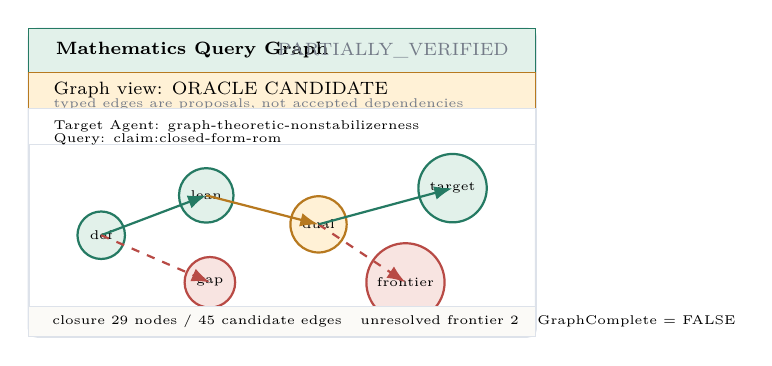
\begin{tikzpicture}[>=Latex,scale=0.92,transform shape]
        \draw[rounded corners=3pt,fill=white,draw=line,thick] (0,0) rectangle (7.0,4.25);
        \draw[fill=greenlite,draw=green] (0,3.65) rectangle (7.0,4.25);
        \node[anchor=west,font=\scriptsize\bfseries] at (0.25,3.95) {Mathematics Query Graph};
        \node[anchor=east,font=\scriptsize\color{muted}] at (6.75,3.95) {PARTIALLY\_VERIFIED};
        \draw[fill=amberlite,draw=amber] (0,3.15) rectangle (7.0,3.65);
        \node[anchor=west,font=\scriptsize] at (0.22,3.4) {Graph view: ORACLE CANDIDATE};
        \node[anchor=west,font=\tiny\color{muted}] at (0.22,3.2) {typed edges are proposals, not accepted dependencies};
        \draw[fill=white,draw=line] (0,2.65) rectangle (7.0,3.15);
        \node[anchor=west,font=\tiny] at (0.22,2.9) {Target Agent: graph-theoretic-nonstabilizerness};
        \node[anchor=west,font=\tiny] at (0.22,2.72) {Query: claim:closed-form-rom};
        \foreach \p/\t/\fill/\drawc in {(1.0,1.4)/def/greenlite/green,(2.45,1.95)/lean/greenlite/green,(2.5,0.75)/gap/redlite/red,(4.0,1.55)/dual/amberlite/amber,(5.2,0.75)/frontier/redlite/red,(5.85,2.05)/target/greenlite/green}
          \node[circle,fill=\fill,draw=\drawc,thick,minimum size=0.45cm,font=\tiny] at \p {\t};
        \draw[->,green,thick] (1.0,1.4) -- (2.45,1.95);
        \draw[->,red,dashed,thick] (1.0,1.4) -- (2.5,0.75);
        \draw[->,amber,thick] (2.45,1.95) -- (4.0,1.55);
        \draw[->,red,dashed,thick] (4.0,1.55) -- (5.2,0.75);
        \draw[->,green,thick] (4.0,1.55) -- (5.85,2.05);
        \draw[fill=paper,draw=line] (0,0) rectangle (7.0,0.42);
        \node[anchor=west,font=\tiny] at (0.2,0.21) {closure 29 nodes / 45 candidate edges \quad unresolved frontier 2 \quad GraphComplete = FALSE};
      \end{tikzpicture}
    \column{0.34\textwidth}
      \textbf{Legend}
      \begin{itemize}\setlength{\itemsep}{0.3em}
        \item green: linked to a Lean declaration
        \item blue: definition / theorem interface
        \item yellow: candidate / scope / local delta
        \item red: gap, frontier, or known counterexample
      \end{itemize}
      \vspace{0.25em}
      \colorbox{redlite}{\parbox{0.95\linewidth}{\centering\scriptsize Red is not one failure mode:\\distinguish GAP, PROOF\_GAP, BLOCKED, and FALSE.}}
  \end{columns}
  \source{Simplified read-only demo; d3-dag computes the candidate backward closure.}
\end{frame}

\section{Iteration log}

\begin{frame}{Iteration 0: split a compound theorem into interfaces}
  \begin{columns}[T,onlytextwidth]
    \column{0.52\textwidth}
      \begin{block}{Input}
        One compound theorem mixes a projected polytope, sign constraints, linear-program duality, graph equivalence, and a closed form in one paragraph.
      \end{block}
      \vspace{0.45em}
      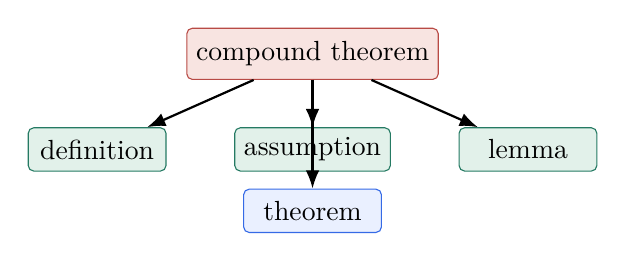
\begin{tikzpicture}[>=Latex,node distance=0.42cm and 0.55cm]
        \node[rounded corners=2pt,fill=redlite,draw=red,minimum width=2.5cm,minimum height=0.65cm,align=center] (all) {compound theorem};
        \node[rounded corners=2pt,fill=greenlite,draw=green,minimum width=1.75cm,minimum height=0.55cm,align=center,below left=0.6cm and 0.25cm of all] (d) {definition};
        \node[rounded corners=2pt,fill=greenlite,draw=green,minimum width=1.75cm,minimum height=0.55cm,align=center,below=0.6cm of all] (a) {assumption};
        \node[rounded corners=2pt,fill=greenlite,draw=green,minimum width=1.75cm,minimum height=0.55cm,align=center,below right=0.6cm and 0.25cm of all] (l) {lemma};
        \node[rounded corners=2pt,fill=bluelite,draw=blue,minimum width=1.75cm,minimum height=0.55cm,align=center,below=1.38cm of all] (t) {theorem};
        \draw[->,thick] (all) -- (d);
        \draw[->,thick] (all) -- (a);
        \draw[->,thick] (all) -- (l);
        \draw[->,thick] (all) -- (t);
      \end{tikzpicture}
    \column{0.43\textwidth}
      \textbf{Every node carries at least:}
      \begin{itemize}\setlength{\itemsep}{0.3em}
        \item source anchor
        \item normalized statement
        \item quantifiers / domain / assumptions
        \item exactness and scope
        \item downstream blockers
      \end{itemize}
      \vspace{0.25em}
      \tagbox{amberlite}{Keep undefined claims explicit; do not fill gaps with prose.}
  \end{columns}
  \source{AgtXIv Mathematics Pipeline: strict mathematical claim decomposition.}
\end{frame}

\begin{frame}{Iteration 1: build a high-recall candidate graph}
  \begin{center}
    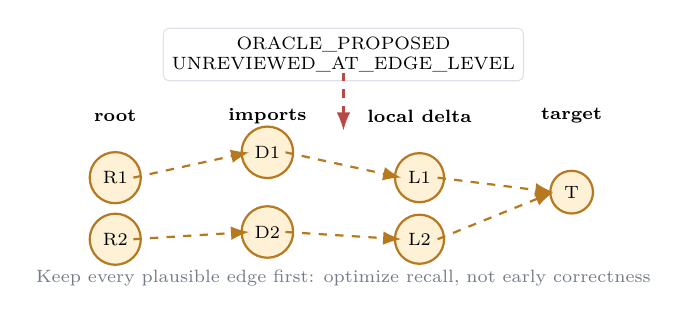
\begin{tikzpicture}[>=Latex,scale=0.92,transform shape]
      \foreach \x/\lab in {0/root,2.1/imports,4.2/local delta,6.3/target}
        \node[font=\scriptsize\bfseries] at (\x,2.05) {\lab};
      \foreach \x/\y/\labnode in {0/1.2/R1,0/0.35/R2,2.1/1.55/D1,2.1/0.45/D2,4.2/1.2/L1,4.2/0.35/L2,6.3/1.0/T}
        \node[circle,fill=amberlite,draw=amber,thick,minimum size=0.5cm,font=\scriptsize] at (\x,\y) {\labnode};
      \draw[->,dashed,amber,thick] (0.25,1.2) -- (1.85,1.55);
      \draw[->,dashed,amber,thick] (0.25,0.35) -- (1.85,0.45);
      \draw[->,dashed,amber,thick] (2.35,1.55) -- (3.95,1.2);
      \draw[->,dashed,amber,thick] (2.35,0.45) -- (3.95,0.35);
      \draw[->,dashed,amber,thick] (4.45,1.2) -- (6.05,1.0);
      \draw[->,dashed,amber,thick] (4.45,0.35) -- (6.05,1.0);
      \node[rounded corners=2pt,fill=white,draw=line,align=center,font=\scriptsize] at (3.15,2.9)
        {ORACLE\_PROPOSED\\UNREVIEWED\_AT\_EDGE\_LEVEL};
      \draw[->,red,dashed,thick] (3.15,2.65) -- (3.15,1.85);
      \node[font=\scriptsize\color{muted},align=center] at (3.15,-0.18)
        {Keep every plausible edge first: optimize recall, not early correctness};
    \end{tikzpicture}
  \end{center}
  \vspace{0.45em}
  \centering\tagbox{amberlite}{green / red are first-pass display states, not scientific acceptance.}
  \source{graph\_view = ORACLE\_CANDIDATE; edges remain candidates until source and Lean alignment.}
\end{frame}

\begin{frame}{Iteration 2: align sources and connect Lean declarations}
  \begin{columns}[T,onlytextwidth]
    \column{0.54\textwidth}
      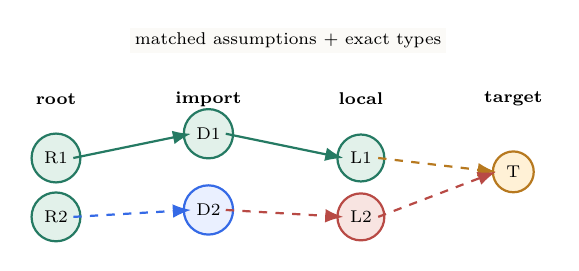
\begin{tikzpicture}[>=Latex,scale=0.88,transform shape]
        \foreach \x/\lab in {0/root,2.2/import,4.4/local,6.6/target}
          \node[font=\scriptsize\bfseries] at (\x,2.05) {\lab};
        \foreach \x/\y/\labnode/\fill/\drawc in {0/1.2/R1/greenlite/green,0/0.35/R2/greenlite/green,2.2/1.55/D1/greenlite/green,2.2/0.45/D2/bluelite/blue,4.4/1.2/L1/greenlite/green,4.4/0.35/L2/redlite/red,6.6/1.0/T/amberlite/amber}
          \node[circle,fill=\fill,draw=\drawc,thick,minimum size=0.52cm,font=\scriptsize] at (\x,\y) {\labnode};
        \draw[->,green,thick] (0.25,1.2) -- (1.95,1.55);
        \draw[->,blue,dashed,thick] (0.25,0.35) -- (1.95,0.45);
        \draw[->,green,thick] (2.45,1.55) -- (4.15,1.2);
        \draw[->,red,dashed,thick] (2.45,0.45) -- (4.15,0.35);
        \draw[->,amber,dashed,thick] (4.65,1.2) -- (6.35,1.0);
        \draw[->,red,dashed,thick] (4.65,0.35) -- (6.35,1.0);
        \node[font=\scriptsize,align=center,fill=paper,inner sep=2pt] at (3.35,2.9)
          {matched assumptions + exact types};
      \end{tikzpicture}
    \column{0.40\textwidth}
      \begin{itemize}\setlength{\itemsep}{0.35em}
        \item green: linked to a Lean declaration
        \item blue: source-aligned, but no reusable Lean bridge yet
        \item red: GAP / unresolved / blocked
        \item yellow: target's local delta is still unimplemented
      \end{itemize}
      \vspace{0.25em}
      \colorbox{amberlite}{\parbox{0.95\linewidth}{\centering\scriptsize This answers what connects formally,\\not whether the physics and source meanings fully agree.}}
  \end{columns}
  \source{Lean-linked means declaration mapping, not verified coverage.}
\end{frame}

\begin{frame}{Iteration 3: critical audit separates failure modes}
  \begin{columns}[T,onlytextwidth]
    \column{0.48\textwidth}
      \begin{block}{V-representation: proof gap}
        \centering
        \tagbox{redlite}{PROOF\_GAP}\quad
        \tagbox{amberlite}{THEOREM\_NOT\_REFUTED}\quad
        \tagbox{greenlite}{CONDITIONAL\_REPAIR}
      \end{block}
      \vspace{0.4em}
      \small An intermediate bijection in the appendix fails. The registry records an independent repair route and two open premises; it does not claim the theorem is refuted.
    \column{0.48\textwidth}
      \begin{block}{Fixed window: counterexample}
        \centering
        \tagbox{redlite}{FALSE}\quad
        \tagbox{redlite}{EXPLICIT\_COUNTEREXAMPLE}
      \end{block}
      \vspace{0.4em}
      \small For a fixed measurement window $M$, a one-qubit Clifford counterexample increases reduced RoM. That is different from a V-representation proof gap.
  \end{columns}
  \vspace{0.35em}
  \begin{center}
    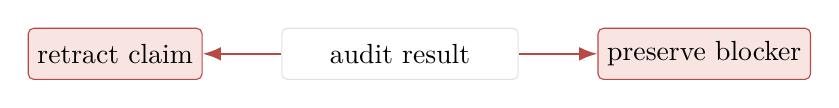
\begin{tikzpicture}[>=Latex]
      \node[rounded corners=2pt,fill=white,draw=line,minimum width=3.0cm,minimum height=0.65cm] (q) {audit result};
      \node[rounded corners=2pt,fill=redlite,draw=red,minimum width=2.2cm,minimum height=0.65cm,right=1.0cm of q] (gap) {preserve blocker};
      \node[rounded corners=2pt,fill=redlite,draw=red,minimum width=2.2cm,minimum height=0.65cm,left=1.0cm of q] (false) {retract claim};
      \draw[->,thick,red] (q) -- (gap);
      \draw[->,thick,red] (q) -- (false);
    \end{tikzpicture}
  \end{center}
  \source{Audit facts: Stabilizerness/AGTXIV\_IMPLEMENTATION.md and registry blocker/status fields.}
\end{frame}

\begin{frame}{Iteration 4: prove only the local delta, then recompute closure}
  \begin{center}
    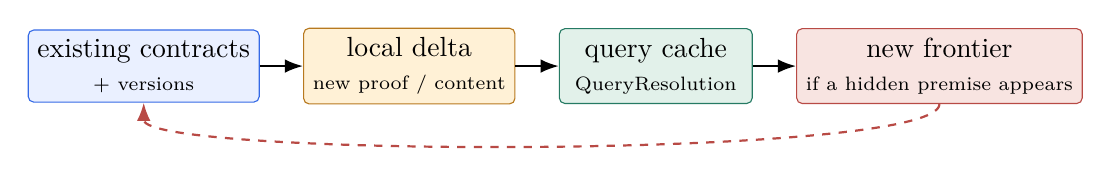
\begin{tikzpicture}[>=Latex,node distance=0.55cm]
      \node[rounded corners=2pt,fill=bluelite,draw=blue,minimum width=2.45cm,minimum height=0.65cm,align=center] (old) {existing contracts\\\scriptsize + versions};
      \node[rounded corners=2pt,fill=amberlite,draw=amber,minimum width=2.45cm,minimum height=0.65cm,align=center,right=of old] (delta) {local delta\\\scriptsize new proof / content};
      \node[rounded corners=2pt,fill=greenlite,draw=green,minimum width=2.45cm,minimum height=0.65cm,align=center,right=of delta] (cache) {query cache\\\scriptsize QueryResolution};
      \node[rounded corners=2pt,fill=redlite,draw=red,minimum width=2.45cm,minimum height=0.65cm,align=center,right=of cache] (front) {new frontier\\\scriptsize if a hidden premise appears};
      \draw[->,thick] (old) -- (delta);
      \draw[->,thick] (delta) -- (cache);
      \draw[->,thick] (cache) -- (front);
      \draw[->,thick,dashed,red] (front.south) .. controls +(0,-0.7) and +(0,-0.7) .. (old.south);
    \end{tikzpicture}
  \end{center}
  \vspace{0.9em}
  \begin{columns}[T,onlytextwidth]
    \column{0.48\textwidth}
      \textbf{Engineering intuition}
      \begin{itemize}\setlength{\itemsep}{0.3em}
        \item A new paper is an increment to a knowledge base, not an isolated PDF.
        \item Verified roots need not be rebuilt.
        \item Implement only the new proof or content needed for the current target.
      \end{itemize}
    \column{0.48\textwidth}
      \textbf{Non-monotonicity matters}
      \begin{itemize}\setlength{\itemsep}{0.3em}
        \item Closing a proof can expose a hidden premise.
        \item The frontier need not shrink every round.
        \item A smaller graph is not the same as truer science.
      \end{itemize}
  \end{columns}
  \source{AgtXIv Mathematics Pipeline: fixed-point reuse and non-promotion.}
\end{frame}

\begin{frame}{The end state is not one Boolean}
  \begin{columns}[T,onlytextwidth]
    \column{0.48\textwidth}
      \begin{block}{Dependency graph complete?}
        \centering\Large\textcolor{red}{FALSE}\par\vspace{0.2em}
        \scriptsize An unresolved external mathematical frontier remains.
      \end{block}
      \vspace{0.25em}
      \begin{block}{Verification closed?}
        \centering\Large\textcolor{red}{FALSE}\par\vspace{0.2em}
        \scriptsize Source, Lean, computational, and physical evidence still need separate acceptance.
      \end{block}
    \column{0.48\textwidth}
      \textbf{Four independent evidence axes}
      \begin{enumerate}\scriptsize\setlength{\itemsep}{0.20em}
        \item source fidelity: what did the source claim?
        \item mathematical correctness: do the assumptions imply the result?
        \item computational reproducibility: do code, data, and environment reproduce it?
        \item physical-semantic alignment: does the formal object match the intended physics?
      \end{enumerate}
      \vspace{0.12em}
      \colorbox{greenlite}{\parbox{0.96\linewidth}{\centering\tiny\textbf{Lean kernel:} the conclusion follows under the encoded definitions and assumptions.}}
  \end{columns}
  \source{The registry can return PARTIALLY\_VERIFIED instead of inventing a global VERIFIED state.}
\end{frame}

\begin{frame}{Takeaway}
  \begin{center}
    {\Large\textbf{A new paper is an increment to a large knowledge base.}}\\[0.8em]
    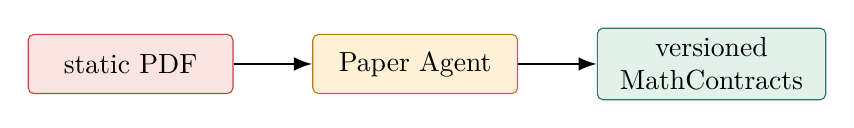
\begin{tikzpicture}[>=Latex]
      \node[rounded corners=2pt,fill=redlite,draw=red,minimum width=2.6cm,minimum height=0.75cm,align=center] (pdf) {static PDF};
      \node[rounded corners=2pt,fill=amberlite,draw=amber,minimum width=2.6cm,minimum height=0.75cm,align=center,right=1.0cm of pdf] (agent) {Paper Agent};
      \node[rounded corners=2pt,fill=greenlite,draw=green,minimum width=2.9cm,minimum height=0.75cm,align=center,right=1.0cm of agent] (mc) {versioned\\MathContracts};
      \draw[->,thick] (pdf) -- (agent);
      \draw[->,thick] (agent) -- (mc);
    \end{tikzpicture}
    \vspace{1.0em}
    \begin{block}{}
      \centering\large Prefer an incomplete path with a visible red frontier\\to a fluent, unauditable ``verified'' answer.
    \end{block}
  \end{center}
  \source{AgtXIv: verification-aware incremental search over scientific claims.}
\end{frame}

\appendix

\begin{frame}{Appendix: arXiv source packages used in this demo}
  \small
  \begin{itemize}\setlength{\itemsep}{0.35em}
    \item Agentic Publication Protocol: \href{https://arxiv.org/abs/2606.27386}{\texttt{arXiv:2606.27386}}\\[-0.1em]
      \scriptsize Source unpacked under \texttt{Reference/Agentic Publication Protocol An Attempt to Modernize Scientific Publication/}.
    \item Multi-agent Autoformalization of Tensor Network Theory: \href{https://arxiv.org/abs/2607.07857}{\texttt{arXiv:2607.07857}}\\[-0.1em]
      \scriptsize Source unpacked under \texttt{Reference/Multi-agent Autoformalization of Tensor Network Theory/}.
    \item Lean-QIT: \href{https://arxiv.org/abs/2607.09632}{\texttt{arXiv:2607.09632}}\\[-0.1em]
      \scriptsize Source unpacked under \texttt{Reference/Lean-QIT Towards a Formal Infrastructure for Quantum Information Theory/}.
    \item End-to-End Formalization of Quantum Error Correction: \href{https://arxiv.org/abs/2605.16523}{\texttt{arXiv:2605.16523}}\\[-0.1em]
      \scriptsize Source unpacked under \texttt{Reference/End-to-End Formalization of Quantum Error Correction/}.
  \end{itemize}
  \vspace{0.5em}
  \scriptsize Related formal-physics identifiers: 2405.08863, 2411.07667, 2601.15737, 2602.16554, 2603.08139, 2607.06379.\\The list avoids presenting ``formal infrastructure'' as one library or one verification standard.
\end{frame}

\end{document}
